\documentclass[abstract=off,10pt,a4paper,bibliography=totocnumbered]{article}
\usepackage[paper=a4paper,left=35mm,right=35mm,top=25mm,bottom=30mm]{geometry}
\usepackage[doublespacing]{setspace}
\usepackage[english]{babel}
\usepackage[utf8]{inputenc}
\usepackage[round]{natbib}
\usepackage{amsmath}
\usepackage{colortbl}
\usepackage{amsfonts}
\usepackage{amssymb}
\usepackage{gensymb}
\usepackage{graphicx}
\usepackage{tikz}
\usepackage{enumerate}
\usepackage{enumitem}
\usepackage{subcaption}
\usepackage{booktabs}
\usepackage[hidelinks]{hyperref}
\usepackage[nameinlink]{cleveref}
\usepackage{lineno}
\usepackage{multirow}
\usepackage{arydshln}
\usepackage[flushleft]{threeparttable}
\usepackage{todonotes}

%------------------------------------------------------------------------------
%	Some Styling
%------------------------------------------------------------------------------
% Creating some TikZ styles
\tikzset{
  nonterminal/.style = {rectangle
    , minimum size = 6mm
    , very thick
    , draw = black!
  }
}

% Changing the style of captions in figures etc.
\captionsetup{labelfont=bf, format=plain, font=small}

% For supplementary material
\newcommand{\beginappendix}{%
  \setcounter{table}{0}
  \renewcommand{\thetable}{S\arabic{table}}%
  \setcounter{figure}{0}
  \renewcommand{\thefigure}{S\arabic{figure}}%
  \setcounter{equation}{0}
  \renewcommand{\theequation}{Equation S\arabic{equation}}%
  \setcounter{section}{0}
  \renewcommand{\thesection}{A.\arabic{section}}%
}

%------------------------------------------------------------------------------
%	Titlepage: Header
%------------------------------------------------------------------------------
\title{\textbf{Appendix}\\ Bound within Boundaries: How Well Do Protected Areas
Match Movement Corridors of Their Most Mobile Protected Species?}

% List of Authors
\author{
  David D. Hofmann\textsuperscript{1,\S,*} \and
  Dominik M. Behr\textsuperscript{1,2,*} \and
  John W. McNutt\textsuperscript{2} \and
  Arpat Ozgul\textsuperscript{1} \and
  Gabriele Cozzi\textsuperscript{1,2}
}

% Reduce spacing between authors
\makeatletter
\def\and{%
  \end{tabular}%
  \hskip -0.5em \@plus.17fil\relax
  \begin{tabular}[t]{c}}
\makeatother

% Current Date
\date{\today}

% And here the masterpiece begins
\begin{document}

% Change page numbering
\pagenumbering{gobble}

% Required to be able to cite
\bibliographystyle{apalike}

% Create Titlepage
\maketitle

%------------------------------------------------------------------------------
%	Titlepage: Additional Info
%------------------------------------------------------------------------------
\begin{flushleft}

\vspace{0.5cm}

\textsuperscript{1} Department of Evolutionary Biology and Environmental
Studies, University of Zurich, Winterthurerstarsse 190, 8057 Zurich,
Switzerland.

\textsuperscript{2} Botswana Predator Conservation Trust, Private Bag 13, Maun,
Botswana.

\textsuperscript{\S} Corresponding author (david.hofmann2@uzh.ch)

\textsuperscript{*} Shared first authorship

\vspace{4cm}

\textbf{Running Title:} Connectivity across a Transfrontier Conservation Area.

\vspace{0.5cm}

\textbf{Keywords:} dispersal, habitat selection, integrated step selection
function, Kavango-Zambezi Transfrontier Conservation Area, landscape
connectivity, least-cost corridors, Lycaon pictus, permeability surface,
protected areas, wildlife management

\end{flushleft}

%------------------------------------------------------------------------------
%	Main Text
%------------------------------------------------------------------------------
\newpage

% Change page numbering
\pagenumbering{arabic}

% Create linenumbers
\linenumbers

% Change to appendix counters
\appendix
\beginappendix

%------------------------------------------------------------------------------
%	Appendix S1: Net Squared Displacement
%------------------------------------------------------------------------------
\section{Net Squared Displacement}

\begin{figure}[hbpt]
  \begin{center}
    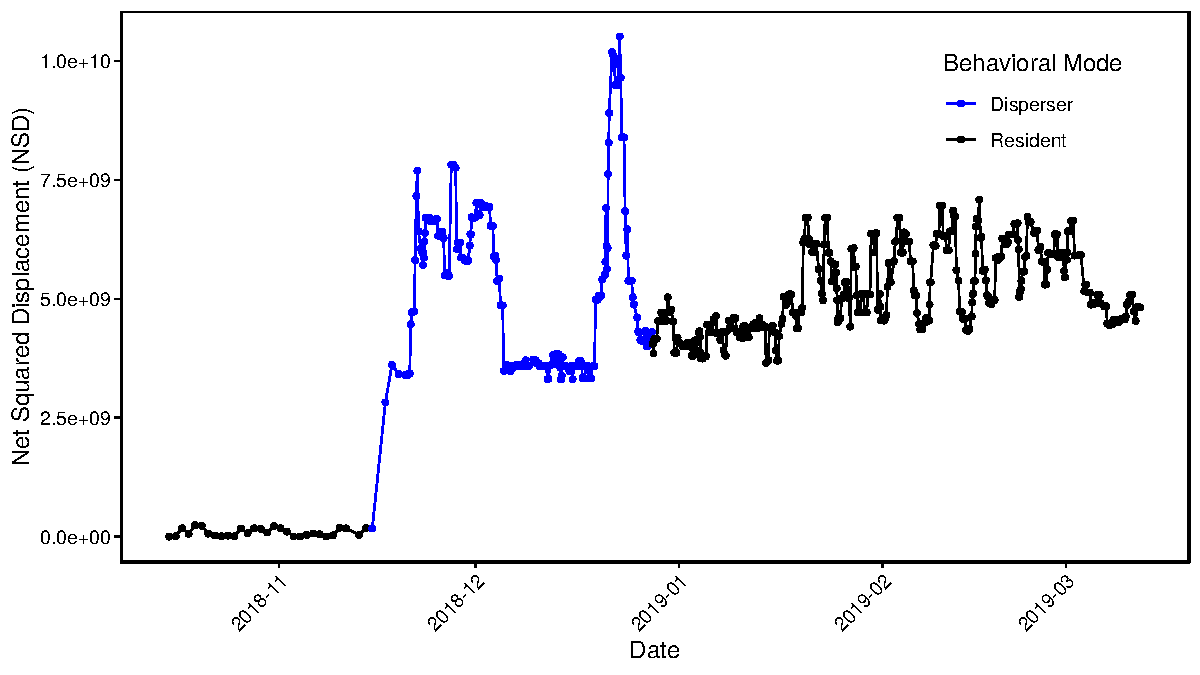
\includegraphics[width = \textwidth]{99_NSD.pdf}
    \caption{NSD displacement through time for one of our dispersers. The blue
    line indicates the period during which we classified the individual as
    dispersing.}
    \label{NSD}
  \end{center}
\end{figure}

%------------------------------------------------------------------------------
%	Appendix S2: GPS Data
%------------------------------------------------------------------------------
\newpage
\newgeometry{left=35mm,right=35mm,top=25mm,bottom=10mm,footskip=0pt}
\section{GPS Data}
\begin{figure}[hbtp]
  \begin{center}
    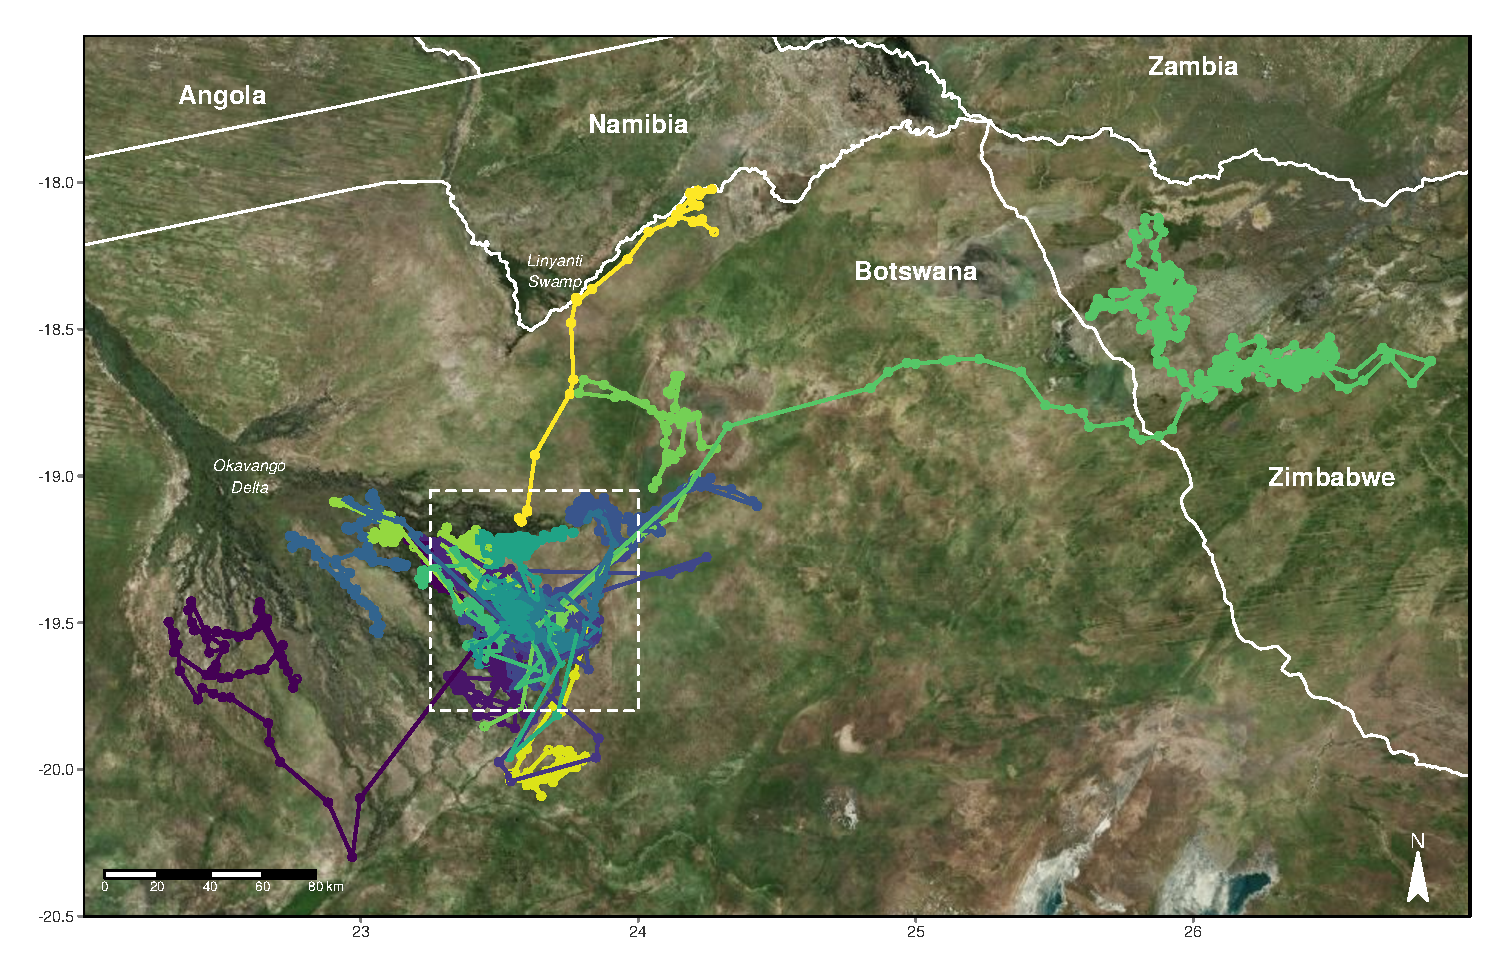
\includegraphics[width = 0.84\textwidth]{99_Trajectories.pdf}
    \caption{Illustration of all trajectories that we recorded. Each color
    represents a different dispersing coalition. All coalitions departed from
    the area which is indicated by the white dashed rectangle. The coalition
    dispersing towards the far east of the map covered over 360 km in under 10
    days. Satellite background imagery was provided by Microsoft Bing.}
    \label{Trajectories}
  \end{center}
\end{figure}

\begin{table}[hbtp]
  \caption{Summary statistics of all GPS relocations that have been recorded on
  dispersing coalitions. The coalition ID refers to the individual in the
  dispersal coalition that was equipped with a GPS collar. All coalitions
  consisted of same-sex individuals.}
  \label{GPSData}
  \begin{center}
    \resizebox{0.95\textwidth}{!}{
      \begin{tabular}{lccccccc}
      \toprule
      \parbox[]{2cm}{\centering Coalition ID} &
        \parbox[]{1cm}{\centering Sex} &
          \parbox[]{2cm}{\centering \ Pack \\ Affiliation} &
            \parbox[]{1.5cm}{\centering \# Fixes \\ Total} &
              \parbox[]{1.5cm}{\centering \# Fixes \\ During \\ Dispersal} &
                \parbox[]{1.5cm}{\centering \# Days \\ Dispersing} &
                  \parbox[]{2cm}{\centering Euclidean \\ Dispersal\\ Distance \\ (in km)} &
                    \parbox[]{2cm}{\centering Cumulative \\ Dispersal \\ Distance \\ (in km)} \\
      \midrule
      Abel & M & MU & 894 & 45 & 9 & 131 & 205 \\
      Amacuro & F & MB & 954 & 583 & 137 & 23 & 1'090 \\
      Belgium & M & ZU & 1'097 & 158 & 28 & 18 & 319 \\
      Dalwhinnie & F & PA & 545 & 62 & 22 & 50 & 243 \\
      Denali & F & MN & 1'096 & 173 & 33 & 11 & 528 \\
      Everest & M & MN & 389 & 123 & 38 & 67 & 572 \\
      Kalahari & F & HT & 1'753 & 467 & 130 & 20 & 1'963 \\
      Karisimbi & M & MN & 438 & 141 & 34 & 45 & 251 \\
      Liuwa & F & AP & 946 & 92 & 19 & 144 & 451 \\
      Lupe & M & KW & 2'209 & 396 & 34 & 8 & 436 \\
      MadameChing & F & AP & 776 & 729 & 136 & 263 & 1'560 \\
      Mirage & M & HT & 814 & 182 & 36 & 7 & 435 \\
      Odzala & M & AP & 1'410 & 205 & 42 & 53 & 412 \\
      Scorpion & M & KB & 2'676 & 393 & 34 & 4 & 471 \\
      Stetson & M & MT & 384 & 383 & 33 & 3 & 481 \\
      Taryn & F & AP & 896 & 37 & 9 & 10 & 130 \\
      \toprule
      \toprule
      \textit{Mean} & - & - & 1'080 & 261 & 48 & 54 & 597 \\
      \textit{(SD)} & - & - & (649) & (207) & (44) & (71) & (508) \\
      \bottomrule
      \end{tabular}
    }
  \end{center}
\end{table}
\restoregeometry

%------------------------------------------------------------------------------
%	Appendix S3: Spatial Covariates
%------------------------------------------------------------------------------
\newpage
\section{Spatial Covariates}
To investigate habitat preferences of dispersing wild dogs, we used a set of
geo-referenced covariates that we aggregated in the categories \textit{land
cover}, \textit{protection status}, and \textit{human influence}. We did not
include any terrain features due to the absence of noteworthy elevational
gradients in our study area. For each covariate, we prepared spatial raster
layers from freely available online services or from remotely sensed satellite
imagery. To ensure a consistent resolution (i.e. cell-size or grain) across
covariates, we coarsened or interpolated all layers to match a resolution of
250m x 250m. We performed processing and manipulation of data as well as all
spatial and statistical analyses using R, version 3.6.1 \citep{R.2019}.

\subsection{Land Cover}
\subsubsection{Water}
The covariate water included rivers, wetlands, and swamps. Because the
inundation extent of the flood in the Okavango Delta is highly variable within
and between years, we created dynamic ``flood maps'' that were updated every
8\textsuperscript{th} day following a remote sensing algorithm developed by the
Okavango Research Institute (ORI; \citealp{Wolski.2017}). To implement the
algorithm, we defined two sets of polygons located in the region of the Okavango
Delta (\Cref{Floodmapping}). The first set consisted of areas known to be
permanent dryland, whereas the second set consisted of permanent waters. Since
we were unable to retrieve the original polygons used in \cite{Wolski.2017}, we
geo-referenced and digitized the polygons reported in their publication. After
recreating the polygons, we used the R-package \textit{getSpatialData}
\citep{Schwalb.2018} to download and pre-process all relatively cloud-free MODIS
Terra images (MCD43A4; \citealp{Schaaf.2015}) available for the period of our
dispersal events. Assessment of cloud cover was based on visual inspection of
MODIS images on ORI's website
(\url{www.okavangodata.ub.bw/ori/monitoring/flood_maps}). After download, we
classified each MODIS image into a binary map of water (flood) and dryland using
a threshold that was identified as follows. First, we extracted all reflectance
values of MODIS Terra Band 7 within the water- and dryland-polygons. Second, we
computed histograms of water-reflectances and dryland-reflectances and
empirically verified that reflectances of the two groups were sufficiently
distinct. More specifically, we checked if superimposing the histograms of
water-reflectances and dryland-reflectances resulted in a bimodal histogram.
This was said to be achieved if the 99\textsuperscript{th} percentile of
water-reflectances did not severely exceed the 1\textsuperscript{st} percentile
of dryland-reflectances (\(p_{0.99, water} - \frac{10}{255} < p_{0.01,
dryland}\)). Third, if bimodality was achieved, we calculated a threshold
(\(t\)) using \ref{EQ1}:

\begin{equation}
\label{EQ1}
t = \widetilde{p}_{water} + 0.3 * (\widetilde{p}_{dryland} -
\widetilde{p}_{water})
\end{equation}

\noindent where \(\widetilde{p}_{water}\) and \(\widetilde{p}_{dryland}\) were
the median reflectances of water and dryland, respectively. We then classified
all pixels of MODIS Terra Band 7 with a value greater than \(t\) as dryland and
all pixels with a value smaller than \(t\) as water.

\begin{figure}[hbtp]
  \begin{center}
    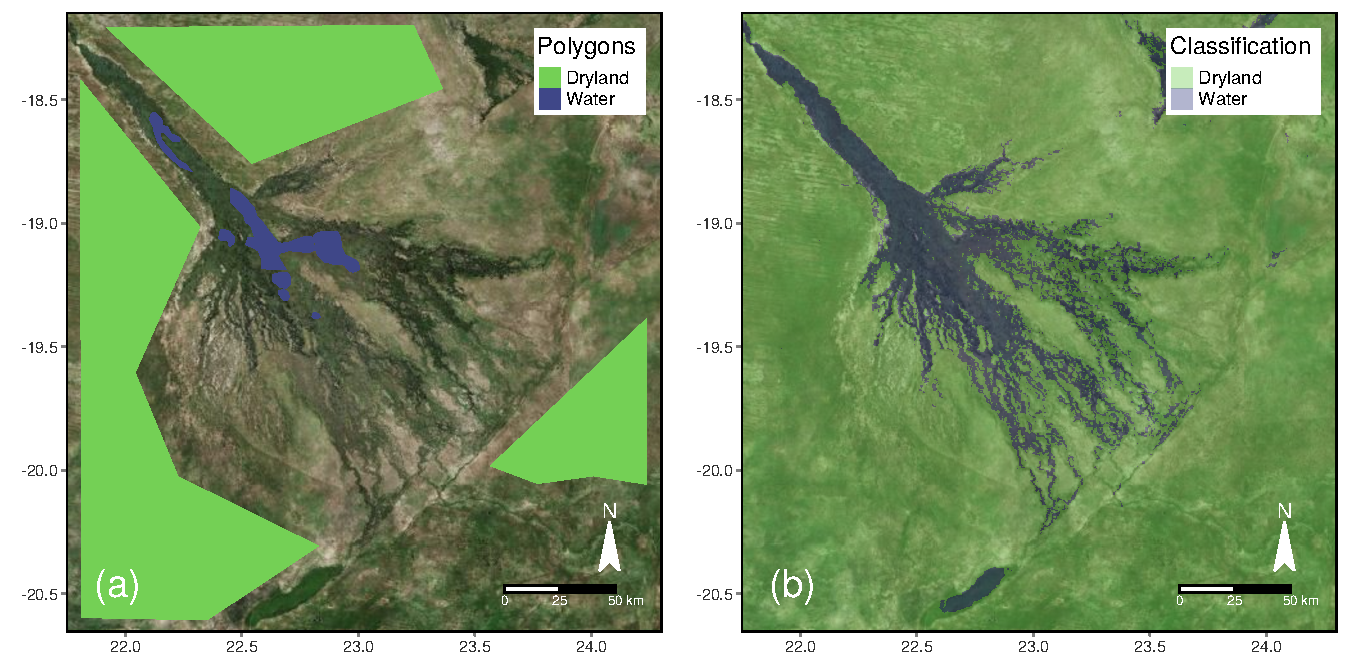
\includegraphics[width = \textwidth]{99_Floodmapping.pdf}
    \caption{Images describing the flood mapping algorithm. (a) The colored
    polygons indicate permanent waters (blue) and permanent dryland (green).
    Below these polygons we extracted reflectance values of MODIS Terra Band 7
    and used their repsective medians to calculate a classification threshold
    \(t\). (b) Example of a classified MODIS Terra Band 7 image after
    application of the threshold. The satellite image in the background was
    provided by Microsoft Bing.}
    \label{Floodmapping}
  \end{center}
\end{figure}

% Dynamic Wetmask
\noindent Importantly, bimodality was not always achieved and in some cases no
flood map could be calculated. In fact, it appears that non-bimodality caused
the ORI algorithm to fail since the end of 2018, which is why no flood maps have
been generated since then (ORI, personal comm.). We hypothesized that this was
caused by the application of static water-polygons that did not cover permanent
waters correctly anymore. Therefore, we revised the algorithm and allowed for a
more dynamic polygonization of water. That is, for each MODIS image we
calculated new water-polygons comprising areas that were covered by the flood in
99\% of the flood maps from the previous five years. All of the necessary flood
maps from previous years were kindly provided to us by ORI. Using this slightly
amended approach, we were able to address some of the bimodality issues and to
classify several additional flood maps for the period of our study. Because
MODIS Terra Band 7 had a resolution of 500m x 500m, we interpolated all maps to
250m x 250m.

% Validation
To validate and compare the performance of our own algorithm to the original
ORI-algorithm, we randomly sampled 48 dates for which ORI prepared classified
images. To make sure that months were equally represented in the sampled dates,
we employed stratified sampling based on months (regardless of the year) and
randomly sampled four maps for each month. For the sampled dates we downloaded
and classified MODIS Terra Band 7 images and compared our classified images to
those provided by ORI (\Cref{FloodmappingValidation}). For each pair of maps we
created a difference map indicating false positives and false negatives and
computed the relative number of wrongly classified pixels. We achieved an
overall accuracy of 97\%, which presumably is an underestimate of the true
performance, as we introduced some errors when resampling the ORI-maps to our
reference grid.

\begin{figure}[hbtp]
  \begin{center}
    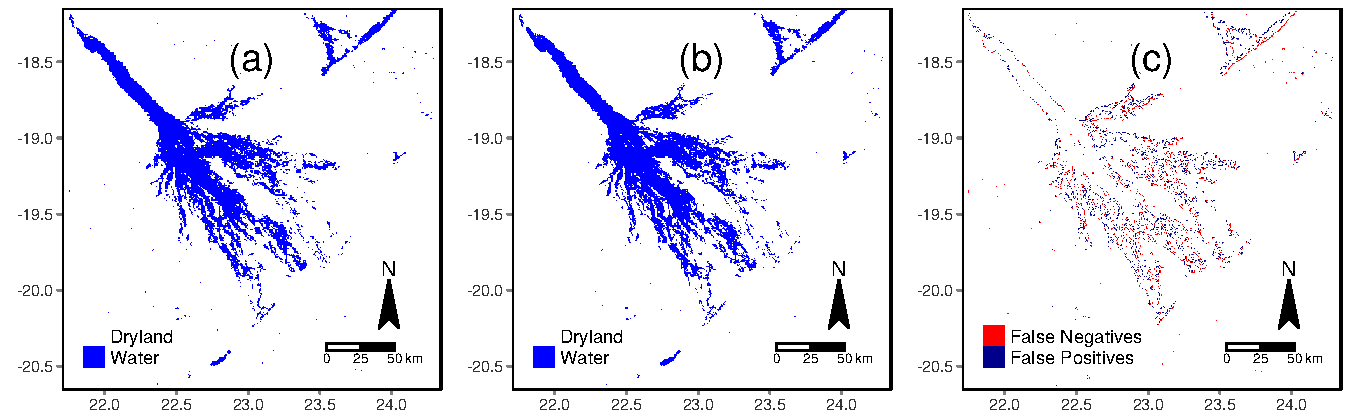
\includegraphics[width = \textwidth]{99_FloodmappingValidation.pdf}
    \caption{Validation procedure of our flood mapping algorithm. (a) Classified
    image that was provided to us by ORI. (b) Image for the same date but now
    classified using our own algorithm. (c) Difference image indicating false
    positives and false negatives in our own classification.}
    \label{FloodmappingValidation}
  \end{center}
\end{figure}

% Static Watermap
\noindent While we created dynamic flood maps for the Okavango Delta, we assumed
the extent of all other water bodies (e.g. Chobe river, Zambezi river) to be
static within and between years. This static representation was based on
Globeland's land cover dataset \citep{Chen.2015}, from which we only retained
the categories \textit{wetland} and \textit{water bodies} and collectively
reclassified them to \textit{water}. Globeland had an original resolution of 30m
x 30m, so we coarsened the layer to 250m x 250m using the mode of each 250m x
250m cell. We further improved river representation by employing the rasterized
MERIT Hydro dataset \citep{Yamazaki.2019} from which we added all rivers with a
width of over 10m to our Globeland layer. We merged dynamic and static water
maps into a large rasterstack, covering the entire study area. We also created a
rasterstack rendering the covariate \textit{distance to water} by calculating
the Euclidean distance of each raster cell in the study area to the nearest
source of water.

\subsubsection{Dryland}
We subdivided dryland into three layers as derived from the MODIS Terra
Vegetation Continuous Fields dataset (MOD44B; \citealp{Dimiceli.2015}). The
three layers depicted percentage cover of tree-vegetation (henceforth
\textit{trees}), non-tree-vegetation (henceforth \textit{shrubs/grassland}), and
non-vegetated (henceforth \textit{bare land}) and added up to 100\% of dryland
coverage. We used our flood map that aligned with the creation date of these
MODIS layers and defined anything covered by water as 0\% vegetated. The MODIS
vegetation layers had a resolution of 250m x 250m and no coarsening or
interpolation was required.

\subsection{Protection Status}
We created a binary layer separating protected from unprotected land. We
downloaded corresponding data on protection status in shapefile format from the
Peace Parks Foundation (\url{www.peaceparks.org}; \citealp{PeaceParks.2019}).
Protected areas included forest reserves, game reserves, wildlife management
areas, and national parks. We classified anything not covered by these
categories as unprotected (e.g. communal pastoral land, private land). We
rasterized the two categories to the binary raster \textit{protection status} (1
= protected, 0 = unprotected) with a resolution of 250m x 250m.

\subsection{Anthropogenic}
We created a raster layer representing human influence by integrating
information on (1) human density, (2) farming, and (3) roads.

\begin{enumerate}[label = (\arabic*)]

  \item We obtained spatial human density estimates through a publicly available
  30m x 30m high-resolution population density dataset
  (\url{www.dataforgood.fb.com}; \citealp{Facebook.2019}). We coarsened the
  layer to 250m x 250m by summing up human density values within each 250m x
  250m cell.

  \item We sourced spatial information on farms from the Globeland
  \citep{Chen.2015} and Cropland \citep{Xiong.2017} land cover datasets from
  which we retained areas that were classified as either \textit{cultivated
  land} or \textit{croplands}. Any other land cover class was not pertinent to
  farming and therefore omitted. Because both layers had a resolution of 30m x
  30m we coarsened them to 250m x 250m by assigning a value of 1 to any 250m x
  250m cell that covered farmland and a value 0 otherwise. Thus, the final layer
  depicted presence (= 1) or absence (= 0) of farms within each 250m x 250m
  cell.

  \item We obtained geo-referenced data on roads from Open Street Map
  \citep{OpenStreetMap.2019}, downloaded through Geofabrik
  (\url{www.geofabrik.de}). We only retained main tarmac roads and omitted
  smaller roads (Table S2) as these are scarcely frequented and do not represent
  an obstacle to wild dog movements \citep{Abrahms.2016}. We rasterized main
  tarmac roads to the binary raster \textit{roads} (1 = roads, 0 = no roads)
  with 250m x 250m resolution. Finally, we created the covariate
  \textit{distance to roads} by calculating the Euclidean distance of each
  raster cell in the study area to the nearest road.

\end{enumerate}

\begin{table}[hbtp]
  \caption{Description of road types, as sourced from Open Street Map's mapping
  guide (\url{https://wiki.openstreetmap.org/wiki/Key:highway}). Roads types
  that were considered for the purpose of this study are shaded in light gray.}
  \label{RoadsDescription}
  \begin{center}
    \resizebox{\textwidth}{!}{
      \begin{tabular}{llp{12cm}}
      \toprule
      Group &
        Subgroup &
          Description \\
      \midrule
      \rowcolor[gray]{0.90}
      Roads &
        motorway &
          A restricted access major divided highway, normally with 2 or more
          running lanes plus emergency hard shoulder. Equivalent to the
          Freeway, Autobahn, etc. \\
      \rowcolor[gray]{0.90}
      Roads &
        trunk &
          The most important roads in a country's system that aren't
          motorways. Need not necessarily be a divided highway. \\
      \rowcolor[gray]{0.90}
      Roads &
        primary &
          The next most important roads in a country's system. Often link
          larger towns. \\
      \rowcolor[gray]{0.90}
      Roads &
        secondary &
          The next most important roads in a country's system. Often link
          towns. \\
      Roads &
        tertiary &
          The next most important roads in a country's system. Often link
          smaller towns and villages \\
      Roads &
        unclassified &
          The least important thorough roads in a country's system, i.e. minor
          roads of a lower classification than tertiary, but which serve a
          purpose other than access to properties. Often link villages and
          hamlets. \\
      Roads &
        residential &
          Roads which serve as an access to housing, without function of
          connecting settlements. Often lined with housing. \\
      Roads &
        service &
          For access roads to, or within an industrial estate, camp site,
          business park, car park etc. \\
      \rowcolor[gray]{0.90}
      Link roads &
        motorway\_link &
          The link roads (sliproads/ramps) leading to/from a motorway from/to
          a motorway or lower class highway. Normally with the same motorway
          restrictions. \\
      \rowcolor[gray]{0.90}
      Link roads &
        trunk\_link &
          The link roads (sliproads/ramps) leading to/from a trunk road
          from/to a trunk road or lower class highway. \\
      \rowcolor[gray]{0.90}
      Link roads &
        primary\_link &
          The link roads (sliproads/ramps) leading to/from a primary road
          from/to a primary road or lower class highway. \\
      \rowcolor[gray]{0.90}
      Link roads &
        secondary\_link &
          The link roads (sliproads/ramps) leading to/from a secondary road
          from/to a secondary road or lower class highway. \\
      Link roads &
        tertiary\_link &
          The link roads (sliproads/ramps) leading to/from a tertiary road
          from/to a tertiary road or lower class highway. \\
      Special road types &
        living\_street &
          For living streets, which are residential streets where pedestrians
          have legal priority over cars, speeds are kept very low and where
          children are allowed to play on the street. \\
      Special road types &
        pedestrian &
          For roads used mainly/exclusively for pedestrians in shopping and
          some residential areas which may allow access by motorised vehicles
          only for very limited periods of the day. \\
      Special road types &
        track &
          Roads for mostly agricultural or forestry uses. \\
      Special road types &
        bus\_guideway &
          A busway where the vehicle is guided by the way (though not a railway)
          and is not suitable for other traffic. \\
      Special road types &
        escape &
          For runaway truck ramps, runaway truck lanes, emergency escape
          ramps, or truck arrester beds. It enables vehicles with braking
          failure to safely stop. \\
      Special road types &
        raceway &
          A course or track for racing \\
      Special road types &
        road &
          A road/way/street/motorway/etc. of unknown type. It can stand for
          anything ranging from a footpath to a motorway. \\
      \bottomrule
      \end{tabular}
    }
  \end{center}
\end{table}

\noindent Because layers (1), (2), and (3) depicted features that are typically
spatially clustered and because not all dispersing coalitions moved within
meaningful distance to each of these features, we totaled values from the layers
describing \textit{human density} (continuous), \textit{farming} (binary), and
\textit{roads} (binary). This approach implied that \textit{roads} and
\textit{farms} entered the final layer with a value of 1, whereas human density
entered the final layer with a value \(\geq 0\) and potentially unbound. To
reduce the influence of outliers in human density estimates, totaled values were
limited to a maximum of 50, which visually resulted in a good balance between
high and low anthropogenic influence and was therefore considered appropriate
for our analysis. To render the fact that humans influence their surroundings
beyond their presence, we followed \cite{Elliot.2014} and applied to each
raster-cell a 5km focal buffer within which we summed up and log-transformed
human-influence values.

\begin{figure}[hbtp]
  \begin{center}
    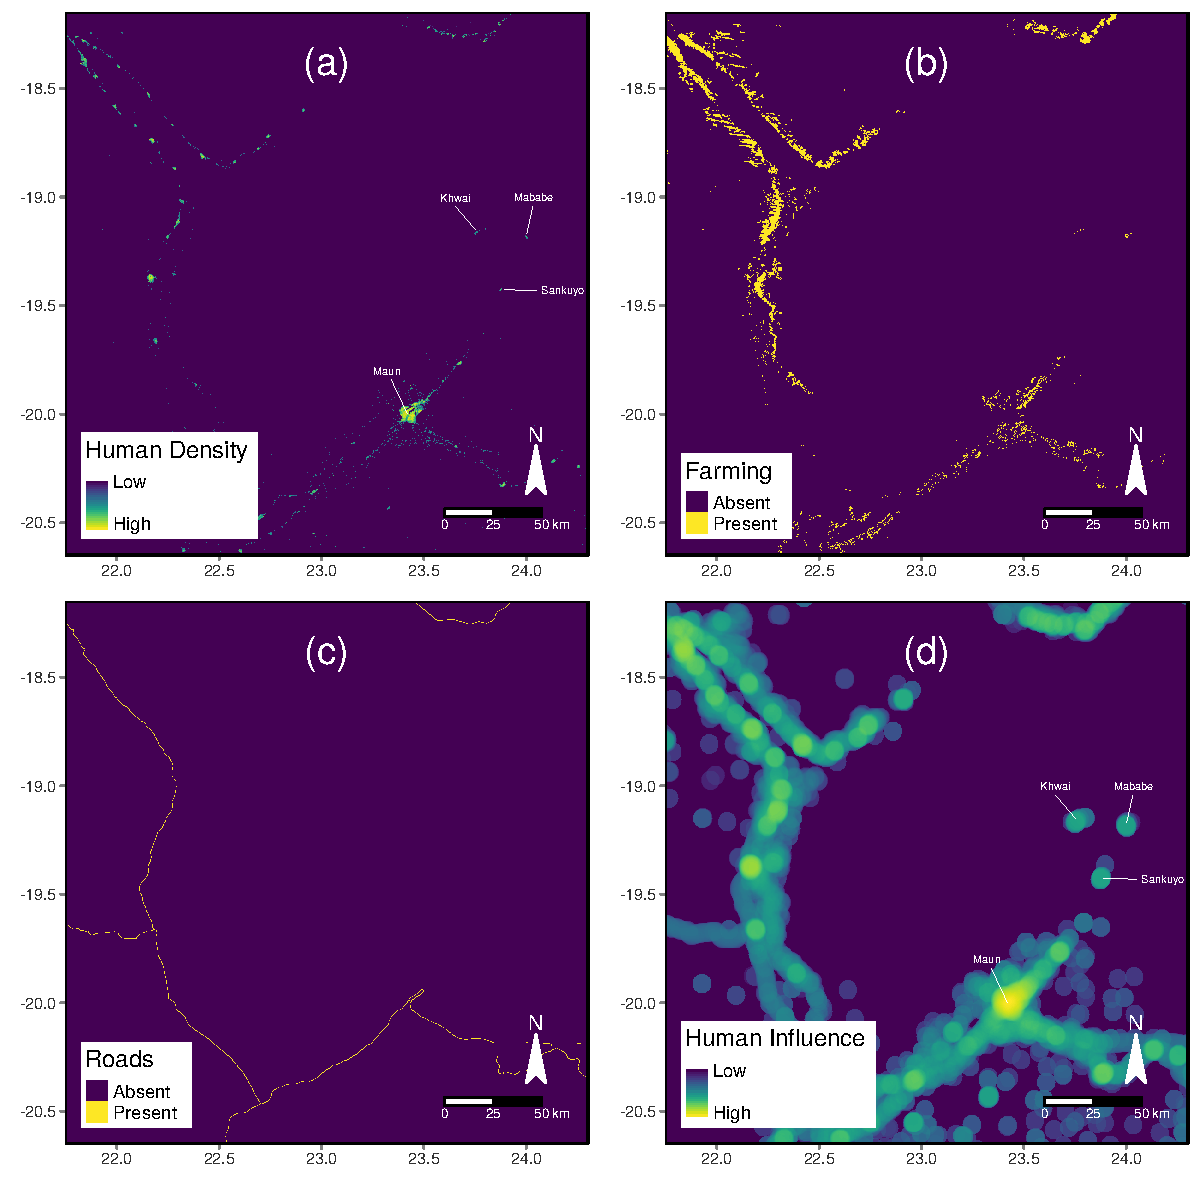
\includegraphics[width = 0.95\textwidth]{99_HumanInfluence.pdf}
    \caption{Sequence of figures that exemplifies how we combined the layers
    (a), (b), and (c) into a single layer for human influence (d). For better
    visibility we show the procedure only for the extent of the Okavango Delta.
    The layer in (a) is based on Facebook's high resolution human density
    dataset (\url{www.dataforgood.fb.com}; \citealp{Facebook.2019}) and depicts
    the estimated number of humans living in each 250m x 250m raster-cell
    (coarsened from 30m x 30m). The layer in (b) is a binary layer and shows
    whether raster-cells are cover any sort of agricultural fields.
    Corresponding data was obtained through the Globeland and Cropland land
    cover datasets \citep{Chen.2015, Xiong.2017}. The layer in (c) shows the
    presence or absence of roads and is based on data from Open Street Map
    \citep{OpenStreetMap.2019}. We merged the layers in (a), (b), and (c) by
    summing up their values, truncating the summed values to a maximum of 50. We
    then log-transforming the values and applied to each raster cell a focal
    buffer of 5km within which we totaled human influence values. The layer in
    (d) depicts the final human influence layer that entered our habitat
    selection model.}
    \label{HumanInfluence}
  \end{center}
\end{figure}

%------------------------------------------------------------------------------
%  Appendix S4: Flood Pulse
%------------------------------------------------------------------------------
\newpage
\section{Typical Flood Pulse}
\begin{figure}[hbtp]
  \begin{center}
    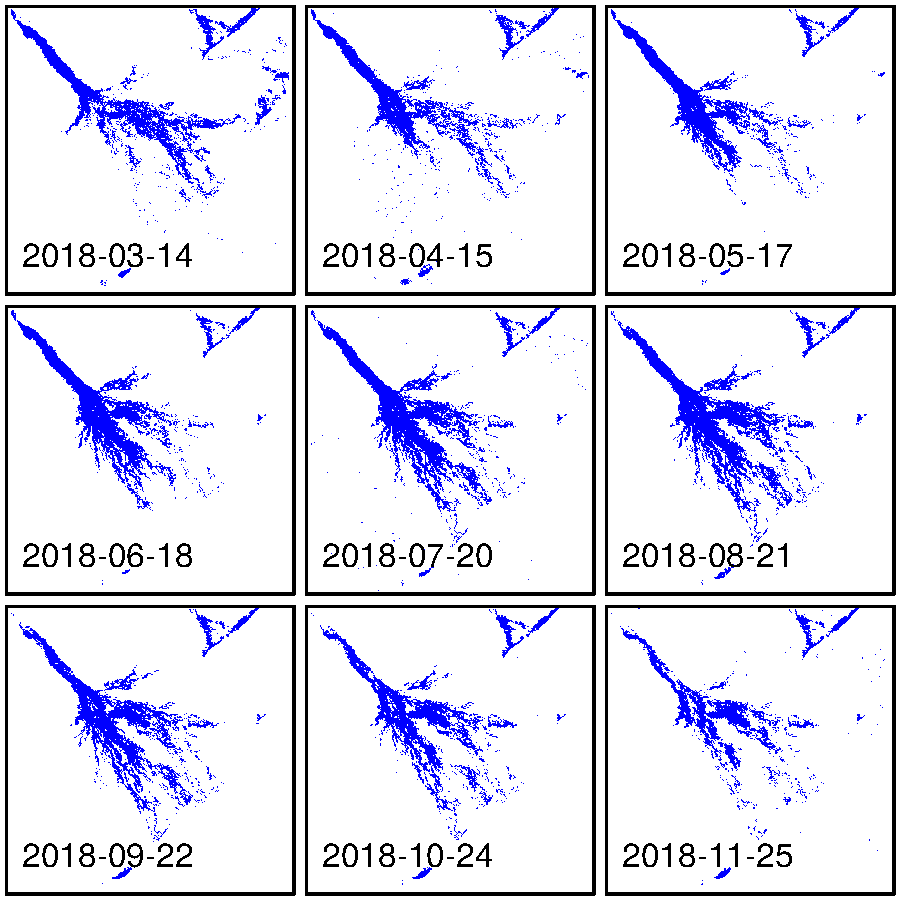
\includegraphics[width = \textwidth]{99_FloodPulse.pdf}
    \caption{Sequence of flood maps showing a typical flood pulse throughout the
    year. The flood arrives from the north-western corner (so called
    ``pan-handle'') of the Okavango Delta and slowly descends through the delta
    in south-eastern direction, where it nourishes several tributaries. The
    extent of the flood peaks around August or September and then slowly
    retracts. Between December and March the reflectance properties of water and
    dryland change, which is why often no accurate flood maps can be obtained
    for these months using remote sensing techniques \citep{Wolski.2017}.}
    \label{FloodPulse}
  \end{center}
\end{figure}

%------------------------------------------------------------------------------
%  Appendix S5: Step Selection Analysis
%------------------------------------------------------------------------------
\newpage
\section{Integrated Step Selection Function}
We used an integrated step selection function (iSSF; \citealp{Avgar.2016}) to
investigate dispersers' selection or avoidance of spatial covariates. In the
iSSF framework, covariates experienced along realized steps are contrasted with
covariates experienced along alternative random steps that the animal could have
taken but decided not to. A step in this framework is defined as the connecting
line between two consecutive GPS relocations \citep{Turchin.1998}. In contrast
to regular SSFs, iSSFs require to include movement metrics as covariates in the
corresponding conditional logistic regression model. Their inclusion, in turn,
allows simultaneous inference on habitat and movement preferences, as well as to
reduce potential biases in estimated habitat preferences \citep{Forester.2009,
Warton.2013, Avgar.2016}.

To conduct iSSF analysis, we followed the recommendations described in Appendix
S1 of the publication by \cite{Avgar.2016}. We prepared our GPS relocation data
for iSSF-analysis using the R-package \textit{amt} \citep{Amt.2019} and coerced
relocations recorded during dispersal to steps that were regularly spaced four
hours apart. Steps that were separated by more than four hours (e.g. due to GPS
failure) were omitted from further analysis (allowing for a minor mismatch of up
to 15 minutes). Each remaining step was paired with 24 random steps, generated
by sampling turning angles from a uniform distribution U(\(-\pi, \pi\)) and step
lengths from a gamma distribution that was fitted using realized step lengths
(shape = 0.3677, scale = 6'302). Together, a realized and its 24 associated
random steps formed a stratum of 25 steps that received a unique identifier.

We extracted spatial covariates along realized and random steps
(\Cref{Appendix:Sources}). For continuous covariates, we calculated the average
value, for categorical covariates the percentage cover along the step. We
further derived a binary variable indicating whether a step crossed a road. We
square-rooted extracted values to render a decreasing marginal impact of
distance. We scaled covariates using a z-score transformation and screened for
correlation using Pearson's Correlation Coefficient. None of the covariates were
overly correlated (\(|r| > 0.6\); \citealp{Latham.2011}) and we retained all of
them for modeling. Despite the covariates mentioned in \Cref{Appendix:Sources},
we included two movement metrics, namely the cosine of the turning angle
(\(cos(ta)\)) and the logarithm of the step length (\(log(sl)\)) in our
regression model \citep{Avgar.2016}. The movement metric \(cos(ta)\) serves to
describe the directionality of a step, as it transforms the circular measure of
(\(-\pi\) to \(\pi\)) into a linear measure (-1, 1). Thus, positive values
indicate forward movements, whereas negative values indicated backward movements
\citep{Turchin.1998}. The movement metric \(log(sl)\), on the other hand, is as
an indicator of the preferred step length. Since in our case steps were spaced
by four hours, \(log(sl)\) can also be interpreted as movement rate.

\begin{table}[hbtp]
  \begin{center}
    \caption{Overview of spatial covariates and their sources. We extracted
    covariates along realized and random steps. For continuous covariates we
    calculated average values along steps, for categorical covariates the
    percentage coverage along steps. We also prepared two covariates indicating
    the distance to water and distance to roads, respectively. We square-rooted
    the values for these two covariates to render a decreasing marginal impact
    of the effect of distance. Finally, we derived a binary indicator of whether
    a step crossed a road or not.}
    \label{Appendix:Sources}
    \resizebox{\textwidth}{!} {
      \begin{threeparttable}
        \begin{tabular}{lllll}
        \hline
        Category &
          Covariate &
            Description &
              Values &
                Source \\
        \midrule
        \multirow{5}{*}{Land Cover}
          & Water
            & Percentage cover of water
              & 0-100\%
                & (1) (2) (3) \\
          & Dryland*
            & Percentage cover of dryland
              & 0-100\%
                & (1) (2) (3) \\
          & DistanceToWater
            & Average distance to nearest water source
              & \(\geq\) 0m
                & (1) (2) (3) \\
          & Shrubs/Grassland
            & Average non-tree vegetation
              & 0-100\%
                & (4) \\
          & Trees
            & Average tree-vegetation
              & 0-100\%
                & (4) \\
          & Bareland*
            & Average non-vegetated area
              & 0-100\%
                & (4) \\
        \hdashline
        \multirow{2}{*}{Protection Status}
          & Protected
            & Percentage cover of protected area
              & 0-100\%
                & (5) \\
          & Unprotected*
            & Percentage cover of unprotected area
              & 0-100\%
                & (5) \\
        \hdashline
        \multirow{3}{*}{Anthropogenic}
          & Human Influence
            & Average human influence
              & \(\geq\) 0
                & (1) (6) (7) (8)\\
          & DistanceToRoads
            & Average distance to nearest road
              & \(\geq\) 0m
                & (1) (6) (7) (8)\\
          & RoadCrossing
            & Binary; whether a step crossed a road
              & 0, 1
                & (1) (6) (7) (8)\\
        \hline
        \end{tabular}
        \begin{tablenotes}
          \item \textit{Sources:} (1) \cite{Chen.2015} (2) \cite{Schaaf.2015}
          (3) \cite{Yamazaki.2019} (4) \cite{Dimiceli.2015} (5)
          \cite{PeaceParks.2019} (6) \cite{Facebook.2019} (7)
          \cite{OpenStreetMap.2019} (8) \cite{Xiong.2017}
          \item
          \item \textit{* Note:} The covariates \textit{Water} and
          \textit{Dryland} added up to 100\%, which is why only \textit{Water}
          was included as explanatory variable in our models. The same applied
          for the group \textit{Shrubs/Grassland}, \textit{Trees}, and
          \textit{Bareland}, where we omitted \textit{Bareland} for modeling.
          Finally, from the group \textit{Protected} and \textit{Unprotected},
          we only included \textit{Protected} in our models.
        \end{tablenotes}
      \end{threeparttable}
    }
  \end{center}
\end{table}

\noindent We then used the iSSF framework to parameterize a habitat selection
model that further served to predict landscape permeability. This habitat
selection model operated under the assumption that dispersing wild dogs assigned
a selection score \(w(x)\) of the following exponential form to each realized
and random step:

\begin{equation}
\label{EQ2}
  w(x) = exp(\beta_1 x_1 + \beta_2 x_2 + ... + \beta_n x_n)
\end{equation}

\noindent That is, the selection score \(w(x)\) of a step depended on its
associated covariates (\(x_1, x_2, ..., x_n\)), as well as on the animal's
preferences for these covariates (\(\beta_1, \beta_2, ..., \beta_n\)). The
probability that a step \(i\) was realized \(P(Y_{i} = 1\)) was then contingent
on the step's selection score, as well as on the selection scores of all
alternative steps in the stratum:

\begin{equation}
\label{EQ3}
  P(Y_{i} = 1 | Y_{1} + Y_{2} + ... + Y_{i} = 1) =
  \frac{w(x_{i})}{w(x_{1}) + w(x_{2}) + ... + w(x_{i})}
\end{equation}

\noindent Habitat and movement preferences of interest, i.e. the \(\beta\)'s,
were then estimated by comparing realized (scored 1) and random (scored 0) steps
in a conditional logistic regression model \citep{Fortin.2005}. In this model,
positive \(\beta\)-coefficients indicate selection of a covariate, negative
\(\beta\)-coefficients avoidance of a covariate. To deal with multiple
individuals, we applied mixed effects conditional logistic regression analysis
following \cite{Muff.2020}. We implemented their method using the R-package
\textit{glmmTMB} \citep{Mollie.2017} and used dispersing coalition ID to model
random intercepts and slopes.

We defined the movement metrics \(cos(ta)\) and \(log(sl)\) as core covariates
and ran forward model selection based on Akaike's Information Criterion (AIC;
\citealp{Burnham.2002}) for all other covariates. We ranked models according to
AIC, assessed relative model weights, and identified the most parsimonious
model. Due to convergence issues, we were unable to model interactions between
covariates.

To validate the predictive power of the most parsimonious habitat selection
model, we ran k-fold cross-validation for case-control studies as described in
\cite{Fortin.2009}. Using 80\% of randomly selected strata, we parameterized a
habitat selection model and predicted selection scores \(w(x)\) for all steps in
the remaining 20\% of strata. According to predicted selection scores we
assigned ranks 1-25 within each stratum, with rank 1 indicating the highest
selection score. We identified the realized step's rank in each stratum and
tallied rank frequencies of realized steps across all strata. Finally, we
carried out a Spearman-rank correlation analysis between ranks and associated
frequencies and we recorded the correlation coefficient (\(r_{s, realized}\)).
We repeated this procedure 100 times with replacement and computed the mean
correlation coefficient (\(\bar{r}_{s, realized}\)), as well as its 95\%
confidence interval. For comparison, we also repeated the same procedure 100
times assuming completely randomized preferences. We implemented randomized
preferences by omitting the realized step from each stratum and identifying the
rank of a randomly chosen random step within each stratum (now only ranks 1-24).
Again, we calculated Spearman's rank correlation coefficient (\(r_{s,
random}\)), its mean across repetitions (\(\bar{r}_{s, random}\)), and its 95\%
confidence interval. Ultimately, the validation proved a significant prediction
in case the confidence intervals of \(\bar{r}_{s, realized}\) and \(\bar{r}_{s,
random}\) did not overlap.

%------------------------------------------------------------------------------
%  Appendix S6: Least Cost Paths and Least Cost Corridors
%------------------------------------------------------------------------------
\newpage
\section{Identification of Least-Cost Paths \& Corridors}
\subsection{Least-Cost Paths}
We implemented factorial LCP analysis between source points using the R-package
\textit{gdistance} (Figure S.7; \citealp{vanEtten.2017}). The package translated
the (unscaled) permeability surface into a network of nodes to find shortest
effective distances between source points based on probabilities of moving from
cell to cell. In our case, the transition probability of moving between two
adjacent cells depended on their averaged permeability. We allowed individuals
to move from each cell to the cell's eight surrounding neighbors (i.e. Moores
neighborhood) and applied a geographic correction to account for the fact that
diagonal neighbors were more remote than orthogonal neighbors. Because African
wild dogs have been observed to cover large dispersal distances
\citep{DaviesMostert.2012, Masenga.2016, Cozzi.2020}, we did not limit LCPs to a
maximal effective cost. After computation, we tallied overlapping LCPs and
identified high-frequency routes.

\subsection{Least-Cost Corridors}
We calculated factorial LCCs \citep{Pinto.2009, Sawyer.2011, Elliot.2014}, again
using the R-package \textit{gdistance} (Figure S.7; \citealp{vanEtten.2017}). To
identify LCCs, we first computed for each source point a cumulative cost map,
which indicated the total minimal costs required to get from the source point to
any other location in the study area. We then obtained an LCC between two source
points by adding up their cumulative cost maps and masking out all cell-values
exceeding the lowest cell-value by more than 5\% \citep{Pinto.2009}. We repeated
this procedure for each possible unique pairwise combination of source points
and thereby identified LCCs between all 68 selected source points. We normalized
the resulting corridor-maps to range from zero to one and tallied them into a
single connectivity map.

\begin{figure}[hbtp]
  \begin{center}
  \begin{minipage}{.32\linewidth}
    \begin{subfigure}[t]{\linewidth}
        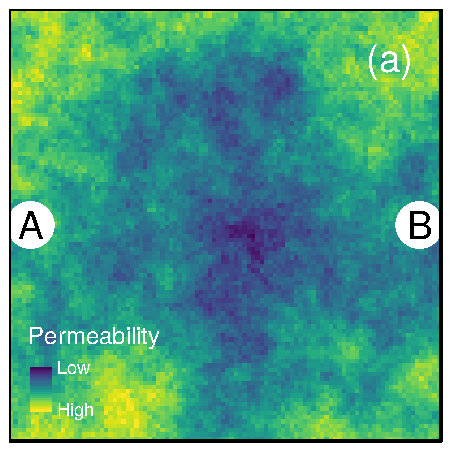
\includegraphics[width=\textwidth]{99_LeastCostPaths(Example1).pdf}
    \end{subfigure}
  \end{minipage}
  \begin{minipage}{.32\linewidth}
    \begin{subfigure}[t]{\linewidth}
        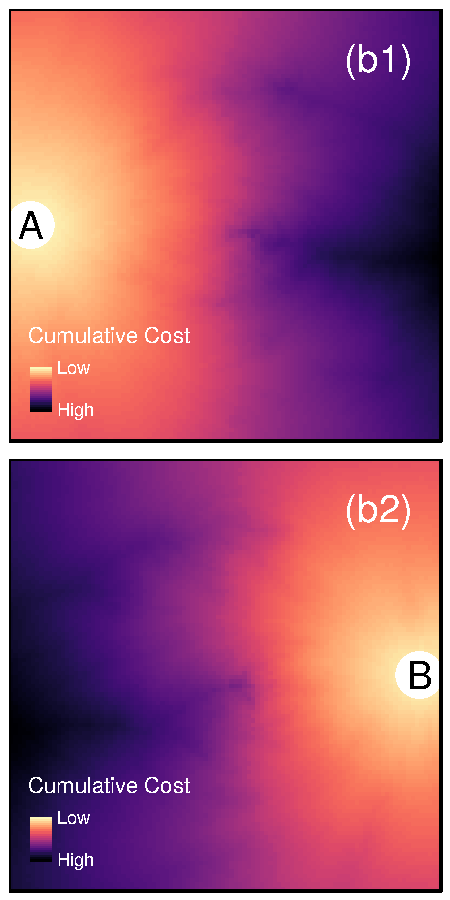
\includegraphics[width=\textwidth]{99_LeastCostPaths(Example2).pdf}
    \end{subfigure}
  \end{minipage}
  \begin{minipage}{.32\linewidth}
    \begin{subfigure}[t]{\linewidth}
        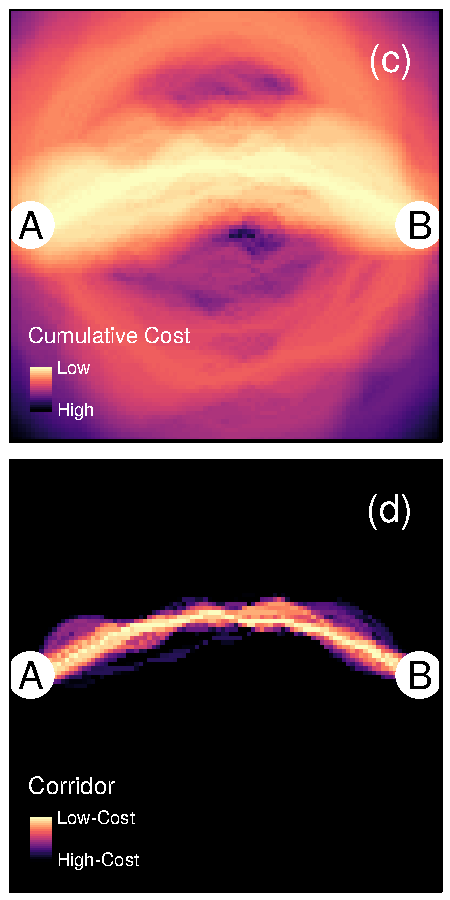
\includegraphics[width=\textwidth]{99_LeastCostPaths(Example3).pdf}
    \end{subfigure}
  \end{minipage}
  \caption{Images illustrating the process of identifying a least-cost corridor
  between source points A and B following \cite{Pinto.2009}. (a) Example of a
  permeability surface, which determines the costs of movement. (b1) Cumulative
  cost map for point A, depicting the total minimal costs necessary to get from
  point A to every other location. (b2) Cumulative cost map for point B,
  depicting the total minimal costs to get from point B to every other location.
  (c) Summed cost maps of points A and B. (d) Masked out corridor containing
  pixels that do not exceed the cheapest pixel by more than 5\%.}
  \label{LCCExample}
  \end{center}
\end{figure}

%------------------------------------------------------------------------------
%  Appendix S7: AIC Model Selection
%------------------------------------------------------------------------------
\newpage
\section{Model Selection Results}
\begin{table}[hbpt]
  \caption{Results from the forward model selection procedure based on Akaike's
  Information Criterion (AIC; \citealp{Burnham.2002}) for the habitat selection
  model. The most parsimonious model outperformed all other models (\(\Delta AIC
  > \) 2) and received a weight of one.}
  \label{ModelAICs}
  \begin{center}
    \resizebox{\textwidth}{!}{
      \begin{threeparttable}
        \begin{tabular}{lllll}
        \toprule
          Covariates & AIC & \(\Delta\)AIC & Weight & LogLik \\
          \midrule
          cos(ta) + sl + log(sl) + W + T + DTW + HI + S & 90068.15 & 0.00 & 1.00 & -45017.08 \\
          cos(ta) + sl + log(sl) + W + T + DTW + HI & 90071.84 & 3.69 & 0.00 & -45020.92 \\
          cos(ta) + sl + log(sl) + W + T + DTW + HI + S + DTR & 90071.94 & 3.79 & 0.00 & -45016.97 \\
          cos(ta) + sl + log(sl) + W + T + DTW + HI + S + P & 90071.94 & 3.79 & 0.00 & -45016.97 \\
          cos(ta) + sl + log(sl) + W + T + DTW + HI + S + RC & 90073.46 & 5.30 & 0.00 & -45015.73 \\
          cos(ta) + sl + log(sl) + W + T + DTW + HI + DTR & 90075.66 & 7.50 & 0.00 & -45020.83 \\
          cos(ta) + sl + log(sl) + W + T + DTW + HI + P & 90075.66 & 7.51 & 0.00 & -45020.83 \\
          cos(ta) + sl + log(sl) + W + T + DTW + HI + S + DTR + P & 90075.79 & 7.64 & 0.00 & -45016.89 \\
          cos(ta) + sl + log(sl) + W + T + DTW + S & 90076.71 & 8.56 & 0.00 & -45023.36 \\
          cos(ta) + sl + log(sl) + W + T + DTW + HI + RC & 90076.84 & 8.69 & 0.00 & -45019.42 \\
          cos(ta) + sl + log(sl) + W + T + DTW + HI + S + DTR + RC & 90077.20 & 9.05 & 0.00 & -45015.60 \\
          cos(ta) + sl + log(sl) + W + T + DTW & 90080.08 & 11.92 & 0.00 & -45027.04 \\
          cos(ta) + sl + log(sl) + W + T + DTW + HI + S + DTR + P + RC & 90080.96 & 12.81 & 0.00 & -45015.48 \\
          cos(ta) + sl + log(sl) + W + T + DTW + DTR & 90082.95 & 14.79 & 0.00 & -45026.47 \\
          cos(ta) + sl + log(sl) + W + T + DTW + P & 90083.31 & 15.16 & 0.00 & -45026.66 \\
          cos(ta) + sl + log(sl) + W + T + HI & 90103.28 & 35.13 & 0.00 & -45038.64 \\
          cos(ta) + sl + log(sl) + W + T & 90109.40 & 41.25 & 0.00 & -45043.70 \\
          cos(ta) + sl + log(sl) + W + T + S & 90110.35 & 42.20 & 0.00 & -45042.17 \\
          cos(ta) + sl + log(sl) + W + T + DTR & 90112.55 & 44.40 & 0.00 & -45043.27 \\
          cos(ta) + sl + log(sl) + W + T + P & 90113.11 & 44.96 & 0.00 & -45043.56 \\
          cos(ta) + sl + log(sl) + W + T + RC & 90113.60 & 45.45 & 0.00 & -45041.80 \\
          cos(ta) + sl + log(sl) + W + DTW & 90118.55 & 50.40 & 0.00 & -45048.28 \\
          cos(ta) + sl + log(sl) + W + HI & 90128.70 & 60.54 & 0.00 & -45053.35 \\
          cos(ta) + sl + log(sl) + W + S & 90132.22 & 64.06 & 0.00 & -45055.11 \\
          cos(ta) + sl + log(sl) + W & 90134.85 & 66.69 & 0.00 & -45058.42 \\
          cos(ta) + sl + log(sl) + W + DTR & 90138.31 & 70.16 & 0.00 & -45058.16 \\
          cos(ta) + sl + log(sl) + W + P & 90138.50 & 70.35 & 0.00 & -45058.25 \\
          cos(ta) + sl + log(sl) + W + RC & 90139.30 & 71.15 & 0.00 & -45056.65 \\
          cos(ta) + sl + log(sl) + S & 90141.98 & 73.83 & 0.00 & -45061.99 \\
          cos(ta) + sl + log(sl) + DTW & 90225.64 & 157.49 & 0.00 & -45103.82 \\
          cos(ta) + sl + log(sl) + T & 90271.73 & 203.58 & 0.00 & -45126.86 \\
          cos(ta) + sl + log(sl) + HI & 90273.18 & 205.02 & 0.00 & -45127.59 \\
          cos(ta) + sl + log(sl) + P & 90285.24 & 217.08 & 0.00 & -45133.62 \\
          cos(ta) + sl + log(sl) + DTR & 90285.33 & 217.18 & 0.00 & -45133.67 \\
          cos(ta) + sl + log(sl) + RC & - & - & - & - \\
          cos(ta) + sl + log(sl) + W + T + DTW + RC & - & - & - & - \\
         \bottomrule
       \end{tabular}
       \begin{tablenotes}
         \item \textit{Note:} W = Water, DTW = Distance To Water, S =
         Shrubs/Grassland, T = Trees, P = Protected, HI = Human Influence, RC =
         Road Crossing, DTR = Distance To Roads. The two models at the bottom
         failed to converge, which is why no AIC value could be obtained.
       \end{tablenotes}
     \end{threeparttable}
    }
  \end{center}
\end{table}

%------------------------------------------------------------------------------
%  Appendix S8: Random Effects Variability
%------------------------------------------------------------------------------
\newpage
\section{Habitat Selection Model: Random Effects}
\begin{figure}[hbtp]
  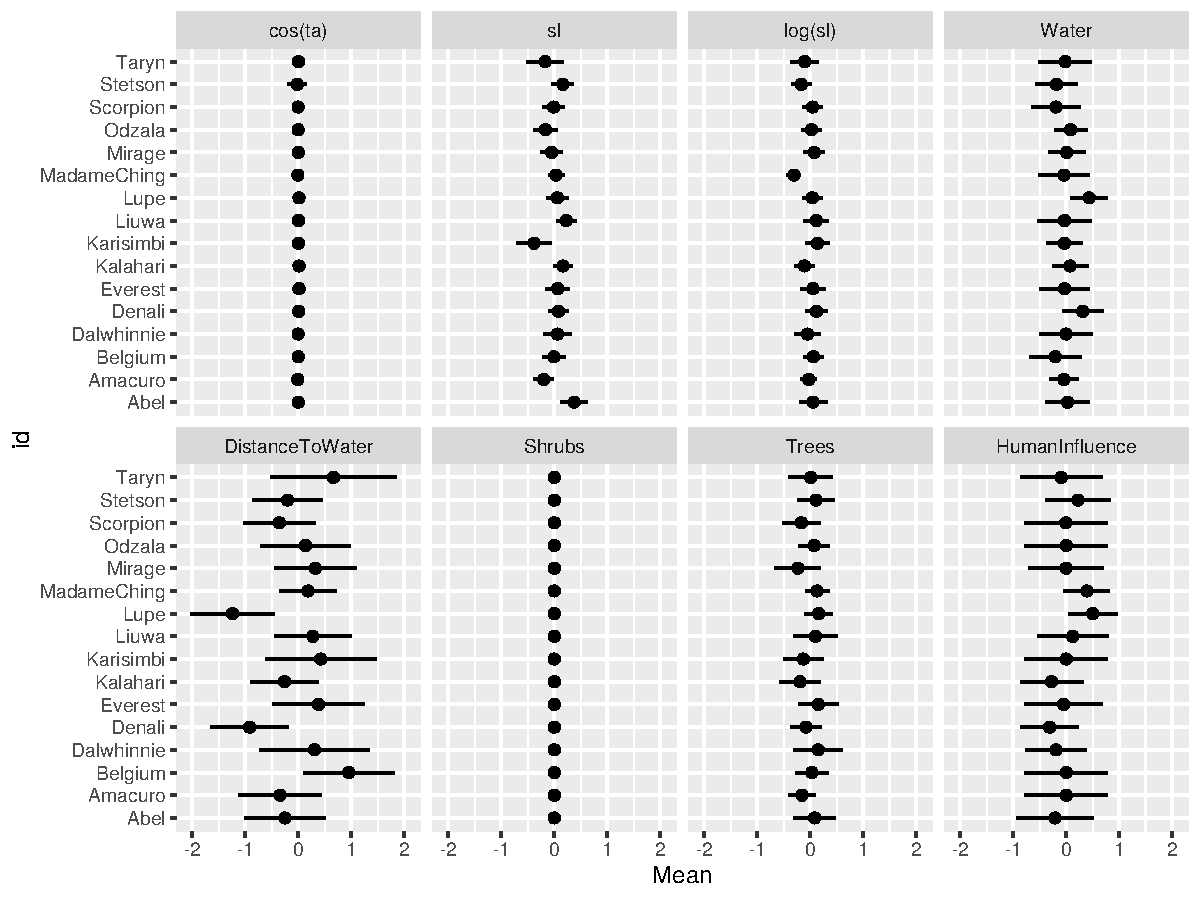
\includegraphics[width = \textwidth]{99_RandomEffects}
  \caption{Plot of random effects showing variability across dispersal
  coalitions. The coalition ID refers to the individual in the dispersal
  coalition that was equipped with a GPS collar.}
  \label{RandomEffects}
\end{figure}

%------------------------------------------------------------------------------
%  Appendix S9: Alternative Source Points
%------------------------------------------------------------------------------
\newpage
\section{Alternative Source Points}
Because we were interested in assessing the sensitivity of our results with
respect to the location of source points, we implemented two competing
approaches to select source points. In a first run, we applied an
omnidirectional \textit{go-through} approach as proposed by \cite{Koen.2014} and
applied by \cite{Pitman.2017}. That is, we distributed 68 equally spaced source
points along the map border and we calculated least-cost paths and least-cost
corridors for all pairwise combinations of them. In contrast to other methods,
this approach has been shown to be less subjective and less sensitive to the
selection of unreasonable source points. Furthermore, such an approach enables
the identification of dispersal routes that do not necessarily connect patches
inhabited by the species. In a second run, we followed the approach described in
\cite{Elliot.2014} and overlayed the study area with a regular grid of points
spaced 100 km apart. From this regular grid we only considered those points that
fell within protected areas \(>\) 700 km\textsuperscript{2}, which conforms with
home-range requirements of African wild dogs \citep{Pomilia.2015}. Finally, we
defined centroids as source points for those protected areas \(>\) 700
km\textsuperscript{2} that were not assigned any source points from the regular
grid. Because wild dogs residing outside of protected areas are rare and
unviable \citep{VanDerMeer.2014}, we consider such a selection of source points
within protected areas to be reasonable. The second procedure also resulted in
68 source points, implying that we calculated 2'278 unique pairwise combinations
and therefore 2'278 unique LCPs and LCCs per approach.
\Cref{AlternativeSourcePoints} illustrates the resulting least-cost paths and
least-cost corridors and highlights that both methods produce qualitatively
similar results. In fact, map values of \Cref{AlternativeSourcePoints} (b1) and
(b2) correlate with \(r\) = 0.86. Nevertheless, one can see that connectivity
following the first approach gets somewhat  ``stretched'' towards the map
borders, which is expected given that the source points are all located at the
borders. Regardless of the method, we find that the major dispersal corridors
run within the borders of the KAZA-TFCA and that mainly impenetrable landscape
remains beyond its borders.

\begin{figure}[hbtp]
  \begin{center}
  \includegraphics[width = \textwidth]{99_LeastCost_Suppl}
  \caption{Comparison of least-cost paths (a) and least-cost corridors (b) using
  different source points. In subfigures (a1) and (b1), 68 source points were
  placed along the map border (black and white semicircles). In subfigures (a2)
  and (b2), on the other hand, source points (black and white circles) were
  placed in protected areas (gray) that were large enough to sustain viable wild
  dog populations (i.e. larger than 700 km\textsuperscript{2},
  \citep{Pomilia.2015}). Continuous thin black lines indicate the borders of the
  KAZA-TFCA, whereas dashed black lines delineate country-borders. For ease of
  spatial reference, we also labeled some national parks (NPs, in dark-grey).}
  \label{AlternativeSourcePoints}
  \end{center}
\end{figure}

\newpage
\begingroup
\singlespacing
\bibliography{Literatur}
\endgroup

\end{document}
